\documentclass[twoside]{book}

% Packages required by doxygen
\usepackage{fixltx2e}
\usepackage{calc}
\usepackage{doxygen}
\usepackage[export]{adjustbox} % also loads graphicx
\usepackage{graphicx}
\usepackage[utf8]{inputenc}
\usepackage{makeidx}
\usepackage{multicol}
\usepackage{multirow}
\PassOptionsToPackage{warn}{textcomp}
\usepackage{textcomp}
\usepackage[nointegrals]{wasysym}
\usepackage[table]{xcolor}

% Font selection
\usepackage[T1]{fontenc}
\usepackage[scaled=.90]{helvet}
\usepackage{courier}
\usepackage{amssymb}
\usepackage{sectsty}
\renewcommand{\familydefault}{\sfdefault}
\allsectionsfont{%
  \fontseries{bc}\selectfont%
  \color{darkgray}%
}
\renewcommand{\DoxyLabelFont}{%
  \fontseries{bc}\selectfont%
  \color{darkgray}%
}
\newcommand{\+}{\discretionary{\mbox{\scriptsize$\hookleftarrow$}}{}{}}

% Page & text layout
\usepackage{geometry}
\geometry{%
  a4paper,%
  top=2.5cm,%
  bottom=2.5cm,%
  left=2.5cm,%
  right=2.5cm%
}
\tolerance=750
\hfuzz=15pt
\hbadness=750
\setlength{\emergencystretch}{15pt}
\setlength{\parindent}{0cm}
\setlength{\parskip}{3ex plus 2ex minus 2ex}
\makeatletter
\renewcommand{\paragraph}{%
  \@startsection{paragraph}{4}{0ex}{-1.0ex}{1.0ex}{%
    \normalfont\normalsize\bfseries\SS@parafont%
  }%
}
\renewcommand{\subparagraph}{%
  \@startsection{subparagraph}{5}{0ex}{-1.0ex}{1.0ex}{%
    \normalfont\normalsize\bfseries\SS@subparafont%
  }%
}
\makeatother

% Headers & footers
\usepackage{fancyhdr}
\pagestyle{fancyplain}
\fancyhead[LE]{\fancyplain{}{\bfseries\thepage}}
\fancyhead[CE]{\fancyplain{}{}}
\fancyhead[RE]{\fancyplain{}{\bfseries\leftmark}}
\fancyhead[LO]{\fancyplain{}{\bfseries\rightmark}}
\fancyhead[CO]{\fancyplain{}{}}
\fancyhead[RO]{\fancyplain{}{\bfseries\thepage}}
\fancyfoot[LE]{\fancyplain{}{}}
\fancyfoot[CE]{\fancyplain{}{}}
\fancyfoot[RE]{\fancyplain{}{\bfseries\scriptsize Generated by Doxygen }}
\fancyfoot[LO]{\fancyplain{}{\bfseries\scriptsize Generated by Doxygen }}
\fancyfoot[CO]{\fancyplain{}{}}
\fancyfoot[RO]{\fancyplain{}{}}
\renewcommand{\footrulewidth}{0.4pt}
\renewcommand{\chaptermark}[1]{%
  \markboth{#1}{}%
}
\renewcommand{\sectionmark}[1]{%
  \markright{\thesection\ #1}%
}

% Indices & bibliography
\usepackage{natbib}
\usepackage[titles]{tocloft}
\setcounter{tocdepth}{3}
\setcounter{secnumdepth}{5}
\makeindex

% Hyperlinks (required, but should be loaded last)
\usepackage{ifpdf}
\ifpdf
  \usepackage[pdftex,pagebackref=true]{hyperref}
\else
  \usepackage[ps2pdf,pagebackref=true]{hyperref}
\fi
\hypersetup{%
  colorlinks=true,%
  linkcolor=blue,%
  citecolor=blue,%
  unicode%
}

% Custom commands
\newcommand{\clearemptydoublepage}{%
  \newpage{\pagestyle{empty}\cleardoublepage}%
}

\usepackage{caption}
\captionsetup{labelsep=space,justification=centering,font={bf},singlelinecheck=off,skip=4pt,position=top}

%===== C O N T E N T S =====

\begin{document}

% Titlepage & ToC
\hypersetup{pageanchor=false,
             bookmarksnumbered=true,
             pdfencoding=unicode
            }
\pagenumbering{roman}
\begin{titlepage}
\vspace*{7cm}
\begin{center}%
{\Large frontier\+\_\+exploration\+\_\+turtlebot \\[1ex]\large 0.\+1 }\\
\vspace*{1cm}
{\large Generated by Doxygen 1.8.11}\\
\end{center}
\end{titlepage}
\clearemptydoublepage
\tableofcontents
\clearemptydoublepage
\pagenumbering{arabic}
\hypersetup{pageanchor=true}

%--- Begin generated contents ---
\chapter{Class Index}
\section{Class List}
Here are the classes, structs, unions and interfaces with brief descriptions\+:\begin{DoxyCompactList}
\item\contentsline{section}{\hyperlink{classCollisionDetector}{Collision\+Detector} \\*Class to find the the presence of the obstacle and to distinguish the position of the obstance in the front or rear of the turtlebot }{\pageref{classCollisionDetector}}{}
\item\contentsline{section}{\hyperlink{classPathPlanning}{Path\+Planning} \\*\hyperlink{classPathPlanning}{Path\+Planning} Class class to publish spiral trajectories and linear trajectories and kicks in the colloision avoiding algorithm when required }{\pageref{classPathPlanning}}{}
\end{DoxyCompactList}

\chapter{File Index}
\section{File List}
Here is a list of all files with brief descriptions\+:\begin{DoxyCompactList}
\item\contentsline{section}{/home/saurav/ros\+\_\+workspace/src/frontier\+\_\+exploration\+\_\+turtlebot/include/frontier\+\_\+exploration\+\_\+turtlebot/\hyperlink{CollisionDetector_8h}{Collision\+Detector.\+h} \\*\hyperlink{classCollisionDetector}{Collision\+Detector} class declaration Declares functions to publish distance from the obstacle and collision flag }{\pageref{CollisionDetector_8h}}{}
\item\contentsline{section}{/home/saurav/ros\+\_\+workspace/src/frontier\+\_\+exploration\+\_\+turtlebot/include/frontier\+\_\+exploration\+\_\+turtlebot/\hyperlink{PathPlanning_8h}{Path\+Planning.\+h} \\*\hyperlink{classPathPlanning}{Path\+Planning} class declaration Declares functions to publish spiral trajectories }{\pageref{PathPlanning_8h}}{}
\item\contentsline{section}{/home/saurav/ros\+\_\+workspace/src/frontier\+\_\+exploration\+\_\+turtlebot/src/\hyperlink{CollisionDetector_8cpp}{Collision\+Detector.\+cpp} \\*Implements the collision\+Detector class methods }{\pageref{CollisionDetector_8cpp}}{}
\item\contentsline{section}{/home/saurav/ros\+\_\+workspace/src/frontier\+\_\+exploration\+\_\+turtlebot/src/\hyperlink{src_2main_8cpp}{main.\+cpp} }{\pageref{src_2main_8cpp}}{}
\item\contentsline{section}{/home/saurav/ros\+\_\+workspace/src/frontier\+\_\+exploration\+\_\+turtlebot/src/\hyperlink{PathPlanning_8cpp}{Path\+Planning.\+cpp} \\*Implements the \hyperlink{classPathPlanning}{Path\+Planning} class methods }{\pageref{PathPlanning_8cpp}}{}
\item\contentsline{section}{/home/saurav/ros\+\_\+workspace/src/frontier\+\_\+exploration\+\_\+turtlebot/test/\hyperlink{CollisionDetectorTest_8cpp}{Collision\+Detector\+Test.\+cpp} \\*Tests the collision\+Detector class methods }{\pageref{CollisionDetectorTest_8cpp}}{}
\item\contentsline{section}{/home/saurav/ros\+\_\+workspace/src/frontier\+\_\+exploration\+\_\+turtlebot/test/\hyperlink{test_2main_8cpp}{main.\+cpp} }{\pageref{test_2main_8cpp}}{}
\item\contentsline{section}{/home/saurav/ros\+\_\+workspace/src/frontier\+\_\+exploration\+\_\+turtlebot/test/\hyperlink{PathPlanningTest_8cpp}{Path\+Planning\+Test.\+cpp} \\*Tests the \hyperlink{classPathPlanning}{Path\+Planning} class methods }{\pageref{PathPlanningTest_8cpp}}{}
\end{DoxyCompactList}

\chapter{Class Documentation}
\hypertarget{classCollisionDetector}{}\section{Collision\+Detector Class Reference}
\label{classCollisionDetector}\index{Collision\+Detector@{Collision\+Detector}}


class to find the the presence of the obstacle and to distinguish the position of the obstance in the front or rear of the turtlebot  




{\ttfamily \#include $<$Collision\+Detector.\+h$>$}

\subsection*{Public Member Functions}
\begin{DoxyCompactItemize}
\item 
\hyperlink{classCollisionDetector_ab3f66bd8d272a21674e38bf46d4d31e0}{Collision\+Detector} ()
\begin{DoxyCompactList}\small\item\em constructor \hyperlink{classCollisionDetector}{Collision\+Detector} class initializes values of Collision\+Flag to 0 \end{DoxyCompactList}\item 
\hyperlink{classCollisionDetector_a1a0f7a386920e0cf83a101be92f04598}{$\sim$\+Collision\+Detector} ()
\begin{DoxyCompactList}\small\item\em destructor \hyperlink{classCollisionDetector}{Collision\+Detector} class destroys \hyperlink{classCollisionDetector}{Collision\+Detector} class objects when it goes out of scope. \end{DoxyCompactList}\item 
void \hyperlink{classCollisionDetector_af960b1e537e227487ee117d17be962c6}{laser\+Callback} (const sensor\+\_\+msgs\+::\+Laser\+Scan\+::\+Const\+Ptr \&msg)
\begin{DoxyCompactList}\small\item\em laser callback function\+Check \+:A call back function to read laserscan data and checks if the obstacle is within the vicinity of the robot and sets the Collision\+Flag(0,1,2) based on the position of the object \end{DoxyCompactList}\item 
int \hyperlink{classCollisionDetector_a04d7a0db86d2023cbc196fa0831f6dba}{check\+Obstacles} ()
\begin{DoxyCompactList}\small\item\em returns the value stored in Collision\+Flag \end{DoxyCompactList}\end{DoxyCompactItemize}
\subsection*{Private Attributes}
\begin{DoxyCompactItemize}
\item 
int \hyperlink{classCollisionDetector_a9222efa13cfe6db4d1bbbc57e18a9d1e}{Collision\+Flag}
\end{DoxyCompactItemize}


\subsection{Detailed Description}
class to find the the presence of the obstacle and to distinguish the position of the obstance in the front or rear of the turtlebot 

Definition at line 46 of file Collision\+Detector.\+h.



\subsection{Constructor \& Destructor Documentation}
\index{Collision\+Detector@{Collision\+Detector}!Collision\+Detector@{Collision\+Detector}}
\index{Collision\+Detector@{Collision\+Detector}!Collision\+Detector@{Collision\+Detector}}
\subsubsection[{\texorpdfstring{Collision\+Detector()}{CollisionDetector()}}]{\setlength{\rightskip}{0pt plus 5cm}Collision\+Detector\+::\+Collision\+Detector (
\begin{DoxyParamCaption}
{}
\end{DoxyParamCaption}
)}\hypertarget{classCollisionDetector_ab3f66bd8d272a21674e38bf46d4d31e0}{}\label{classCollisionDetector_ab3f66bd8d272a21674e38bf46d4d31e0}


constructor \hyperlink{classCollisionDetector}{Collision\+Detector} class initializes values of Collision\+Flag to 0 


\begin{DoxyParams}{Parameters}
{\em none} & \\
\hline
\end{DoxyParams}
\begin{DoxyReturn}{Returns}
none 
\end{DoxyReturn}


Definition at line 40 of file Collision\+Detector.\+cpp.



References Collision\+Flag.

\index{Collision\+Detector@{Collision\+Detector}!````~Collision\+Detector@{$\sim$\+Collision\+Detector}}
\index{````~Collision\+Detector@{$\sim$\+Collision\+Detector}!Collision\+Detector@{Collision\+Detector}}
\subsubsection[{\texorpdfstring{$\sim$\+Collision\+Detector()}{~CollisionDetector()}}]{\setlength{\rightskip}{0pt plus 5cm}Collision\+Detector\+::$\sim$\+Collision\+Detector (
\begin{DoxyParamCaption}
{}
\end{DoxyParamCaption}
)}\hypertarget{classCollisionDetector_a1a0f7a386920e0cf83a101be92f04598}{}\label{classCollisionDetector_a1a0f7a386920e0cf83a101be92f04598}


destructor \hyperlink{classCollisionDetector}{Collision\+Detector} class destroys \hyperlink{classCollisionDetector}{Collision\+Detector} class objects when it goes out of scope. 


\begin{DoxyParams}{Parameters}
{\em none} & \\
\hline
\end{DoxyParams}
\begin{DoxyReturn}{Returns}
none 
\end{DoxyReturn}


Definition at line 45 of file Collision\+Detector.\+cpp.



\subsection{Member Function Documentation}
\index{Collision\+Detector@{Collision\+Detector}!check\+Obstacles@{check\+Obstacles}}
\index{check\+Obstacles@{check\+Obstacles}!Collision\+Detector@{Collision\+Detector}}
\subsubsection[{\texorpdfstring{check\+Obstacles()}{checkObstacles()}}]{\setlength{\rightskip}{0pt plus 5cm}int Collision\+Detector\+::check\+Obstacles (
\begin{DoxyParamCaption}
{}
\end{DoxyParamCaption}
)}\hypertarget{classCollisionDetector_a04d7a0db86d2023cbc196fa0831f6dba}{}\label{classCollisionDetector_a04d7a0db86d2023cbc196fa0831f6dba}


returns the value stored in Collision\+Flag 


\begin{DoxyParams}{Parameters}
{\em none} & \\
\hline
\end{DoxyParams}
\begin{DoxyReturn}{Returns}
int 
\end{DoxyReturn}


Definition at line 95 of file Collision\+Detector.\+cpp.



References Collision\+Flag.



Referenced by Path\+Planning\+::linear\+Path\+Generator(), Path\+Planning\+::spiral\+Path\+Generator(), and T\+E\+S\+T().

\index{Collision\+Detector@{Collision\+Detector}!laser\+Callback@{laser\+Callback}}
\index{laser\+Callback@{laser\+Callback}!Collision\+Detector@{Collision\+Detector}}
\subsubsection[{\texorpdfstring{laser\+Callback(const sensor\+\_\+msgs\+::\+Laser\+Scan\+::\+Const\+Ptr \&msg)}{laserCallback(const sensor_msgs::LaserScan::ConstPtr &msg)}}]{\setlength{\rightskip}{0pt plus 5cm}void Collision\+Detector\+::laser\+Callback (
\begin{DoxyParamCaption}
\item[{const sensor\+\_\+msgs\+::\+Laser\+Scan\+::\+Const\+Ptr \&}]{msg}
\end{DoxyParamCaption}
)}\hypertarget{classCollisionDetector_af960b1e537e227487ee117d17be962c6}{}\label{classCollisionDetector_af960b1e537e227487ee117d17be962c6}


laser callback function\+Check \+:A call back function to read laserscan data and checks if the obstacle is within the vicinity of the robot and sets the Collision\+Flag(0,1,2) based on the position of the object 


\begin{DoxyParams}{Parameters}
{\em msg} & of type sensor\+\_\+msgs\+::\+Laser\+Scan \\
\hline
\end{DoxyParams}
\begin{DoxyReturn}{Returns}
none 
\end{DoxyReturn}


Definition at line 48 of file Collision\+Detector.\+cpp.



References Collision\+Flag.



Referenced by Path\+Planning\+::\+Path\+Planning(), and T\+E\+S\+T().



\subsection{Member Data Documentation}
\index{Collision\+Detector@{Collision\+Detector}!Collision\+Flag@{Collision\+Flag}}
\index{Collision\+Flag@{Collision\+Flag}!Collision\+Detector@{Collision\+Detector}}
\subsubsection[{\texorpdfstring{Collision\+Flag}{CollisionFlag}}]{\setlength{\rightskip}{0pt plus 5cm}int Collision\+Detector\+::\+Collision\+Flag\hspace{0.3cm}{\ttfamily [private]}}\hypertarget{classCollisionDetector_a9222efa13cfe6db4d1bbbc57e18a9d1e}{}\label{classCollisionDetector_a9222efa13cfe6db4d1bbbc57e18a9d1e}


Definition at line 49 of file Collision\+Detector.\+h.



Referenced by check\+Obstacles(), Collision\+Detector(), and laser\+Callback().



The documentation for this class was generated from the following files\+:\begin{DoxyCompactItemize}
\item 
/home/saurav/ros\+\_\+workspace/src/frontier\+\_\+exploration\+\_\+turtlebot/include/frontier\+\_\+exploration\+\_\+turtlebot/\hyperlink{CollisionDetector_8h}{Collision\+Detector.\+h}\item 
/home/saurav/ros\+\_\+workspace/src/frontier\+\_\+exploration\+\_\+turtlebot/src/\hyperlink{CollisionDetector_8cpp}{Collision\+Detector.\+cpp}\end{DoxyCompactItemize}

\hypertarget{classPathPlanning}{}\section{Path\+Planning Class Reference}
\label{classPathPlanning}\index{Path\+Planning@{Path\+Planning}}


\hyperlink{classPathPlanning}{Path\+Planning} Class class to publish spiral trajectories and linear trajectories and kicks in the colloision avoiding algorithm when required.  




{\ttfamily \#include $<$Path\+Planning.\+h$>$}



Collaboration diagram for Path\+Planning\+:\nopagebreak
\begin{figure}[H]
\begin{center}
\leavevmode
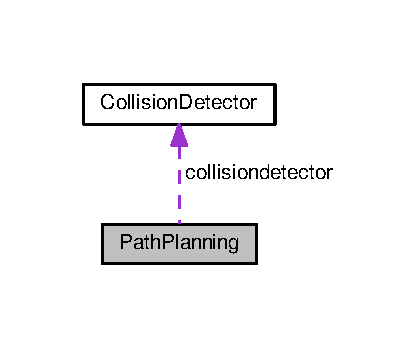
\includegraphics[width=200pt]{classPathPlanning__coll__graph}
\end{center}
\end{figure}
\subsection*{Public Member Functions}
\begin{DoxyCompactItemize}
\item 
\hyperlink{classPathPlanning_a314735f239a01515a3450205dd144619}{Path\+Planning} ()
\begin{DoxyCompactList}\small\item\em constructor \hyperlink{classPathPlanning}{Path\+Planning} class \end{DoxyCompactList}\item 
\hyperlink{classPathPlanning_ab1f231c8ce62aac1f2e9743aa85ba940}{$\sim$\+Path\+Planning} ()
\begin{DoxyCompactList}\small\item\em destructor \hyperlink{classPathPlanning}{Path\+Planning} class \end{DoxyCompactList}\item 
void \hyperlink{classPathPlanning_ab096aae6f4a9636d60f3acdc582a6e4a}{spiral\+Path\+Generator} ()
\begin{DoxyCompactList}\small\item\em spiral generator function \end{DoxyCompactList}\item 
void \hyperlink{classPathPlanning_ac8bdfa5f35d5819bd7981e15b95c637b}{linear\+Path\+Generator} ()
\begin{DoxyCompactList}\small\item\em linear generator function \end{DoxyCompactList}\end{DoxyCompactItemize}
\subsection*{Private Attributes}
\begin{DoxyCompactItemize}
\item 
\hyperlink{classCollisionDetector}{Collision\+Detector} \hyperlink{classPathPlanning_a698ed28a6ed1408f311af37170a180a2}{collisiondetector}
\item 
int \hyperlink{classPathPlanning_a8ffa246d97c8d79cb18a1fd61e805467}{count}
\item 
int \hyperlink{classPathPlanning_a1346e45eb6566236a55b666e350cb62b}{Max\+Count}
\item 
float \hyperlink{classPathPlanning_a88e654d2dffefce6b3253dca0d05af2c}{linear\+Speed}
\item 
float \hyperlink{classPathPlanning_aaa87b2917fd4cc8705601b037458dbec}{angular\+Speed}
\item 
geometry\+\_\+msgs\+::\+Twist \hyperlink{classPathPlanning_adc9393eeed2386dd694935a241d61dc2}{msg}
\item 
ros\+::\+Publisher \hyperlink{classPathPlanning_a95ffa20c78692b3af113a52f37607f23}{pub\+Vel}
\item 
ros\+::\+Node\+Handle \hyperlink{classPathPlanning_a1835423557580f21ff1d569e892cc0d5}{nh}
\item 
ros\+::\+Subscriber \hyperlink{classPathPlanning_ad30204ed2c193139c5d5b3f8ed07bc8d}{sub}
\end{DoxyCompactItemize}


\subsection{Detailed Description}
\hyperlink{classPathPlanning}{Path\+Planning} Class class to publish spiral trajectories and linear trajectories and kicks in the colloision avoiding algorithm when required. 

Definition at line 47 of file Path\+Planning.\+h.



\subsection{Constructor \& Destructor Documentation}
\index{Path\+Planning@{Path\+Planning}!Path\+Planning@{Path\+Planning}}
\index{Path\+Planning@{Path\+Planning}!Path\+Planning@{Path\+Planning}}
\subsubsection[{\texorpdfstring{Path\+Planning()}{PathPlanning()}}]{\setlength{\rightskip}{0pt plus 5cm}Path\+Planning\+::\+Path\+Planning (
\begin{DoxyParamCaption}
{}
\end{DoxyParamCaption}
)}\hypertarget{classPathPlanning_a314735f239a01515a3450205dd144619}{}\label{classPathPlanning_a314735f239a01515a3450205dd144619}


constructor \hyperlink{classPathPlanning}{Path\+Planning} class 


\begin{DoxyParams}{Parameters}
{\em none} & \\
\hline
\end{DoxyParams}
\begin{DoxyReturn}{Returns}
none initializes values of count, Max\+Count, linear\+Speed, angular\+Speec and initializes subscribers and publishers 
\end{DoxyReturn}


Definition at line 39 of file Path\+Planning.\+cpp.



References angular\+Speed, collisiondetector, count, Collision\+Detector\+::laser\+Callback(), linear\+Speed, Max\+Count, msg, nh, pub\+Vel, and sub.

\index{Path\+Planning@{Path\+Planning}!````~Path\+Planning@{$\sim$\+Path\+Planning}}
\index{````~Path\+Planning@{$\sim$\+Path\+Planning}!Path\+Planning@{Path\+Planning}}
\subsubsection[{\texorpdfstring{$\sim$\+Path\+Planning()}{~PathPlanning()}}]{\setlength{\rightskip}{0pt plus 5cm}Path\+Planning\+::$\sim$\+Path\+Planning (
\begin{DoxyParamCaption}
{}
\end{DoxyParamCaption}
)}\hypertarget{classPathPlanning_ab1f231c8ce62aac1f2e9743aa85ba940}{}\label{classPathPlanning_ab1f231c8ce62aac1f2e9743aa85ba940}


destructor \hyperlink{classPathPlanning}{Path\+Planning} class 


\begin{DoxyParams}{Parameters}
{\em none} & \\
\hline
\end{DoxyParams}
\begin{DoxyReturn}{Returns}
none destroys \hyperlink{classPathPlanning}{Path\+Planning} class objects when it goes out of scope. 
\end{DoxyReturn}


Definition at line 63 of file Path\+Planning.\+cpp.



References msg, and pub\+Vel.



\subsection{Member Function Documentation}
\index{Path\+Planning@{Path\+Planning}!linear\+Path\+Generator@{linear\+Path\+Generator}}
\index{linear\+Path\+Generator@{linear\+Path\+Generator}!Path\+Planning@{Path\+Planning}}
\subsubsection[{\texorpdfstring{linear\+Path\+Generator()}{linearPathGenerator()}}]{\setlength{\rightskip}{0pt plus 5cm}void Path\+Planning\+::linear\+Path\+Generator (
\begin{DoxyParamCaption}
{}
\end{DoxyParamCaption}
)}\hypertarget{classPathPlanning_ac8bdfa5f35d5819bd7981e15b95c637b}{}\label{classPathPlanning_ac8bdfa5f35d5819bd7981e15b95c637b}


linear generator function 


\begin{DoxyParams}{Parameters}
{\em none} & \\
\hline
\end{DoxyParams}
\begin{DoxyReturn}{Returns}
none generates linear trajectories and publishes them 
\end{DoxyReturn}


Definition at line 74 of file Path\+Planning.\+cpp.



References angular\+Speed, Collision\+Detector\+::check\+Obstacles(), collisiondetector, linear\+Speed, msg, and pub\+Vel.



Referenced by main(), and T\+E\+S\+T().

\index{Path\+Planning@{Path\+Planning}!spiral\+Path\+Generator@{spiral\+Path\+Generator}}
\index{spiral\+Path\+Generator@{spiral\+Path\+Generator}!Path\+Planning@{Path\+Planning}}
\subsubsection[{\texorpdfstring{spiral\+Path\+Generator()}{spiralPathGenerator()}}]{\setlength{\rightskip}{0pt plus 5cm}void Path\+Planning\+::spiral\+Path\+Generator (
\begin{DoxyParamCaption}
{}
\end{DoxyParamCaption}
)}\hypertarget{classPathPlanning_ab096aae6f4a9636d60f3acdc582a6e4a}{}\label{classPathPlanning_ab096aae6f4a9636d60f3acdc582a6e4a}


spiral generator function 


\begin{DoxyParams}{Parameters}
{\em none} & \\
\hline
\end{DoxyParams}
\begin{DoxyReturn}{Returns}
none generates spiral trajectories and publishes them 
\end{DoxyReturn}


Definition at line 97 of file Path\+Planning.\+cpp.



References angular\+Speed, Collision\+Detector\+::check\+Obstacles(), collisiondetector, count, linear\+Speed, Max\+Count, msg, and pub\+Vel.



Referenced by main(), and T\+E\+S\+T().



\subsection{Member Data Documentation}
\index{Path\+Planning@{Path\+Planning}!angular\+Speed@{angular\+Speed}}
\index{angular\+Speed@{angular\+Speed}!Path\+Planning@{Path\+Planning}}
\subsubsection[{\texorpdfstring{angular\+Speed}{angularSpeed}}]{\setlength{\rightskip}{0pt plus 5cm}float Path\+Planning\+::angular\+Speed\hspace{0.3cm}{\ttfamily [private]}}\hypertarget{classPathPlanning_aaa87b2917fd4cc8705601b037458dbec}{}\label{classPathPlanning_aaa87b2917fd4cc8705601b037458dbec}


Definition at line 58 of file Path\+Planning.\+h.



Referenced by linear\+Path\+Generator(), Path\+Planning(), and spiral\+Path\+Generator().

\index{Path\+Planning@{Path\+Planning}!collisiondetector@{collisiondetector}}
\index{collisiondetector@{collisiondetector}!Path\+Planning@{Path\+Planning}}
\subsubsection[{\texorpdfstring{collisiondetector}{collisiondetector}}]{\setlength{\rightskip}{0pt plus 5cm}{\bf Collision\+Detector} Path\+Planning\+::collisiondetector\hspace{0.3cm}{\ttfamily [private]}}\hypertarget{classPathPlanning_a698ed28a6ed1408f311af37170a180a2}{}\label{classPathPlanning_a698ed28a6ed1408f311af37170a180a2}


Definition at line 50 of file Path\+Planning.\+h.



Referenced by linear\+Path\+Generator(), Path\+Planning(), and spiral\+Path\+Generator().

\index{Path\+Planning@{Path\+Planning}!count@{count}}
\index{count@{count}!Path\+Planning@{Path\+Planning}}
\subsubsection[{\texorpdfstring{count}{count}}]{\setlength{\rightskip}{0pt plus 5cm}int Path\+Planning\+::count\hspace{0.3cm}{\ttfamily [private]}}\hypertarget{classPathPlanning_a8ffa246d97c8d79cb18a1fd61e805467}{}\label{classPathPlanning_a8ffa246d97c8d79cb18a1fd61e805467}


Definition at line 52 of file Path\+Planning.\+h.



Referenced by Path\+Planning(), and spiral\+Path\+Generator().

\index{Path\+Planning@{Path\+Planning}!linear\+Speed@{linear\+Speed}}
\index{linear\+Speed@{linear\+Speed}!Path\+Planning@{Path\+Planning}}
\subsubsection[{\texorpdfstring{linear\+Speed}{linearSpeed}}]{\setlength{\rightskip}{0pt plus 5cm}float Path\+Planning\+::linear\+Speed\hspace{0.3cm}{\ttfamily [private]}}\hypertarget{classPathPlanning_a88e654d2dffefce6b3253dca0d05af2c}{}\label{classPathPlanning_a88e654d2dffefce6b3253dca0d05af2c}


Definition at line 56 of file Path\+Planning.\+h.



Referenced by linear\+Path\+Generator(), Path\+Planning(), and spiral\+Path\+Generator().

\index{Path\+Planning@{Path\+Planning}!Max\+Count@{Max\+Count}}
\index{Max\+Count@{Max\+Count}!Path\+Planning@{Path\+Planning}}
\subsubsection[{\texorpdfstring{Max\+Count}{MaxCount}}]{\setlength{\rightskip}{0pt plus 5cm}int Path\+Planning\+::\+Max\+Count\hspace{0.3cm}{\ttfamily [private]}}\hypertarget{classPathPlanning_a1346e45eb6566236a55b666e350cb62b}{}\label{classPathPlanning_a1346e45eb6566236a55b666e350cb62b}


Definition at line 54 of file Path\+Planning.\+h.



Referenced by Path\+Planning(), and spiral\+Path\+Generator().

\index{Path\+Planning@{Path\+Planning}!msg@{msg}}
\index{msg@{msg}!Path\+Planning@{Path\+Planning}}
\subsubsection[{\texorpdfstring{msg}{msg}}]{\setlength{\rightskip}{0pt plus 5cm}geometry\+\_\+msgs\+::\+Twist Path\+Planning\+::msg\hspace{0.3cm}{\ttfamily [private]}}\hypertarget{classPathPlanning_adc9393eeed2386dd694935a241d61dc2}{}\label{classPathPlanning_adc9393eeed2386dd694935a241d61dc2}


Definition at line 60 of file Path\+Planning.\+h.



Referenced by linear\+Path\+Generator(), Path\+Planning(), spiral\+Path\+Generator(), and $\sim$\+Path\+Planning().

\index{Path\+Planning@{Path\+Planning}!nh@{nh}}
\index{nh@{nh}!Path\+Planning@{Path\+Planning}}
\subsubsection[{\texorpdfstring{nh}{nh}}]{\setlength{\rightskip}{0pt plus 5cm}ros\+::\+Node\+Handle Path\+Planning\+::nh\hspace{0.3cm}{\ttfamily [private]}}\hypertarget{classPathPlanning_a1835423557580f21ff1d569e892cc0d5}{}\label{classPathPlanning_a1835423557580f21ff1d569e892cc0d5}


Definition at line 64 of file Path\+Planning.\+h.



Referenced by Path\+Planning().

\index{Path\+Planning@{Path\+Planning}!pub\+Vel@{pub\+Vel}}
\index{pub\+Vel@{pub\+Vel}!Path\+Planning@{Path\+Planning}}
\subsubsection[{\texorpdfstring{pub\+Vel}{pubVel}}]{\setlength{\rightskip}{0pt plus 5cm}ros\+::\+Publisher Path\+Planning\+::pub\+Vel\hspace{0.3cm}{\ttfamily [private]}}\hypertarget{classPathPlanning_a95ffa20c78692b3af113a52f37607f23}{}\label{classPathPlanning_a95ffa20c78692b3af113a52f37607f23}


Definition at line 62 of file Path\+Planning.\+h.



Referenced by linear\+Path\+Generator(), Path\+Planning(), spiral\+Path\+Generator(), and $\sim$\+Path\+Planning().

\index{Path\+Planning@{Path\+Planning}!sub@{sub}}
\index{sub@{sub}!Path\+Planning@{Path\+Planning}}
\subsubsection[{\texorpdfstring{sub}{sub}}]{\setlength{\rightskip}{0pt plus 5cm}ros\+::\+Subscriber Path\+Planning\+::sub\hspace{0.3cm}{\ttfamily [private]}}\hypertarget{classPathPlanning_ad30204ed2c193139c5d5b3f8ed07bc8d}{}\label{classPathPlanning_ad30204ed2c193139c5d5b3f8ed07bc8d}


Definition at line 66 of file Path\+Planning.\+h.



Referenced by Path\+Planning().



The documentation for this class was generated from the following files\+:\begin{DoxyCompactItemize}
\item 
/home/saurav/ros\+\_\+workspace/src/frontier\+\_\+exploration\+\_\+turtlebot/include/frontier\+\_\+exploration\+\_\+turtlebot/\hyperlink{PathPlanning_8h}{Path\+Planning.\+h}\item 
/home/saurav/ros\+\_\+workspace/src/frontier\+\_\+exploration\+\_\+turtlebot/src/\hyperlink{PathPlanning_8cpp}{Path\+Planning.\+cpp}\end{DoxyCompactItemize}

\chapter{File Documentation}
\hypertarget{CollisionDetector_8h}{}\section{/home/saurav/ros\+\_\+workspace/src/frontier\+\_\+exploration\+\_\+turtlebot/include/frontier\+\_\+exploration\+\_\+turtlebot/\+Collision\+Detector.h File Reference}
\label{CollisionDetector_8h}\index{/home/saurav/ros\+\_\+workspace/src/frontier\+\_\+exploration\+\_\+turtlebot/include/frontier\+\_\+exploration\+\_\+turtlebot/\+Collision\+Detector.\+h@{/home/saurav/ros\+\_\+workspace/src/frontier\+\_\+exploration\+\_\+turtlebot/include/frontier\+\_\+exploration\+\_\+turtlebot/\+Collision\+Detector.\+h}}


\hyperlink{classCollisionDetector}{Collision\+Detector} class declaration Declares functions to publish distance from the obstacle and collision flag.  


{\ttfamily \#include $<$sensor\+\_\+msgs/\+Laser\+Scan.\+h$>$}\\*
Include dependency graph for Collision\+Detector.\+h\+:\nopagebreak
\begin{figure}[H]
\begin{center}
\leavevmode
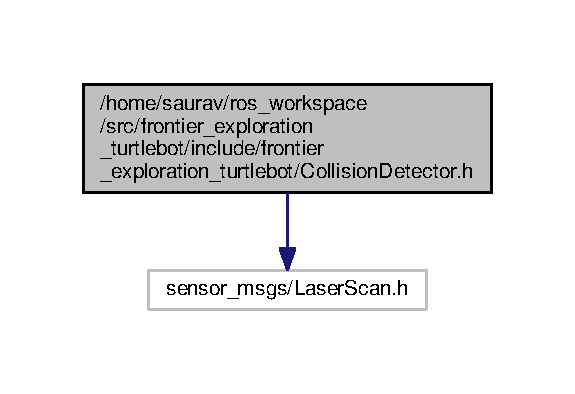
\includegraphics[width=276pt]{CollisionDetector_8h__incl}
\end{center}
\end{figure}
This graph shows which files directly or indirectly include this file\+:\nopagebreak
\begin{figure}[H]
\begin{center}
\leavevmode
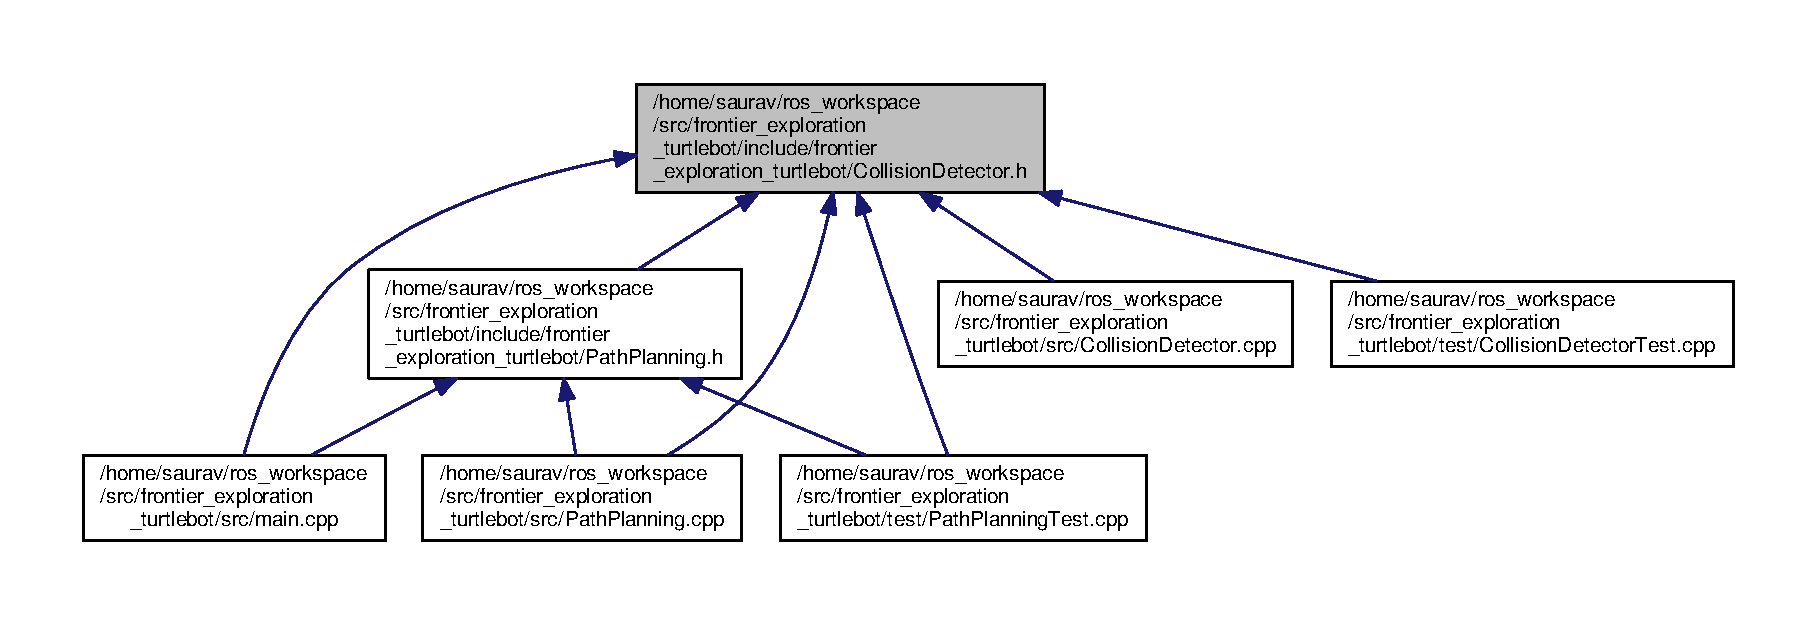
\includegraphics[width=350pt]{CollisionDetector_8h__dep__incl}
\end{center}
\end{figure}
\subsection*{Classes}
\begin{DoxyCompactItemize}
\item 
class \hyperlink{classCollisionDetector}{Collision\+Detector}
\begin{DoxyCompactList}\small\item\em class to find the the presence of the obstacle and to distinguish the position of the obstance in the front or rear of the turtlebot \end{DoxyCompactList}\end{DoxyCompactItemize}


\subsection{Detailed Description}
\hyperlink{classCollisionDetector}{Collision\+Detector} class declaration Declares functions to publish distance from the obstacle and collision flag. 

M\+IT License

Copyright (c) 2018 Saimouli Katragadda, Saurav Kumar

Permission is hereby granted, free of charge, to any person obtaining a copy of this software and associated documentation files (the \char`\"{}\+Software\char`\"{}), to deal in the Software without restriction, including without limitation the rights to use, copy, modify, merge, publish, distribute, sublicense, and/or sell copies of the Software, and to permit persons to whom the Software is furnished to do so, subject to the following conditions\+:

The above copyright notice and this permission notice shall be included in all copies or substantial portions of the Software.

T\+HE S\+O\+F\+T\+W\+A\+RE IS P\+R\+O\+V\+I\+D\+ED \char`\"{}\+A\+S I\+S\char`\"{}, W\+I\+T\+H\+O\+UT W\+A\+R\+R\+A\+N\+TY OF A\+NY K\+I\+ND, E\+X\+P\+R\+E\+SS OR I\+M\+P\+L\+I\+ED, I\+N\+C\+L\+U\+D\+I\+NG B\+UT N\+OT L\+I\+M\+I\+T\+ED TO T\+HE W\+A\+R\+R\+A\+N\+T\+I\+ES OF M\+E\+R\+C\+H\+A\+N\+T\+A\+B\+I\+L\+I\+TY, F\+I\+T\+N\+E\+SS F\+OR A P\+A\+R\+T\+I\+C\+U\+L\+AR P\+U\+R\+P\+O\+SE A\+ND N\+O\+N\+I\+N\+F\+R\+I\+N\+G\+E\+M\+E\+NT. IN NO E\+V\+E\+NT S\+H\+A\+LL T\+HE A\+U\+T\+H\+O\+RS OR C\+O\+P\+Y\+R\+I\+G\+HT H\+O\+L\+D\+E\+RS BE L\+I\+A\+B\+LE F\+OR A\+NY C\+L\+A\+IM, D\+A\+M\+A\+G\+ES OR O\+T\+H\+ER L\+I\+A\+B\+I\+L\+I\+TY, W\+H\+E\+T\+H\+ER IN AN A\+C\+T\+I\+ON OF C\+O\+N\+T\+R\+A\+CT, T\+O\+RT OR O\+T\+H\+E\+R\+W\+I\+SE, A\+R\+I\+S\+I\+NG F\+R\+OM, O\+UT OF OR IN C\+O\+N\+N\+E\+C\+T\+I\+ON W\+I\+TH T\+HE S\+O\+F\+T\+W\+A\+RE OR T\+HE U\+SE OR O\+T\+H\+ER D\+E\+A\+L\+I\+N\+GS IN T\+HE S\+O\+F\+T\+W\+A\+RE.

\begin{DoxyAuthor}{Author}
Saimouli Katragadda 

Saurav Kumar 
\end{DoxyAuthor}
\begin{DoxyCopyright}{Copyright}
M\+IT License 
\end{DoxyCopyright}

\hypertarget{PathPlanning_8h}{}\section{/home/saurav/ros\+\_\+workspace/src/frontier\+\_\+exploration\+\_\+turtlebot/include/frontier\+\_\+exploration\+\_\+turtlebot/\+Path\+Planning.h File Reference}
\label{PathPlanning_8h}\index{/home/saurav/ros\+\_\+workspace/src/frontier\+\_\+exploration\+\_\+turtlebot/include/frontier\+\_\+exploration\+\_\+turtlebot/\+Path\+Planning.\+h@{/home/saurav/ros\+\_\+workspace/src/frontier\+\_\+exploration\+\_\+turtlebot/include/frontier\+\_\+exploration\+\_\+turtlebot/\+Path\+Planning.\+h}}


\hyperlink{classPathPlanning}{Path\+Planning} class declaration Declares functions to publish spiral trajectories.  


{\ttfamily \#include $<$ros/ros.\+h$>$}\\*
{\ttfamily \#include $<$geometry\+\_\+msgs/\+Twist.\+h$>$}\\*
{\ttfamily \#include $<$frontier\+\_\+exploration\+\_\+turtlebot/\+Collision\+Detector.\+h$>$}\\*
Include dependency graph for Path\+Planning.\+h\+:\nopagebreak
\begin{figure}[H]
\begin{center}
\leavevmode
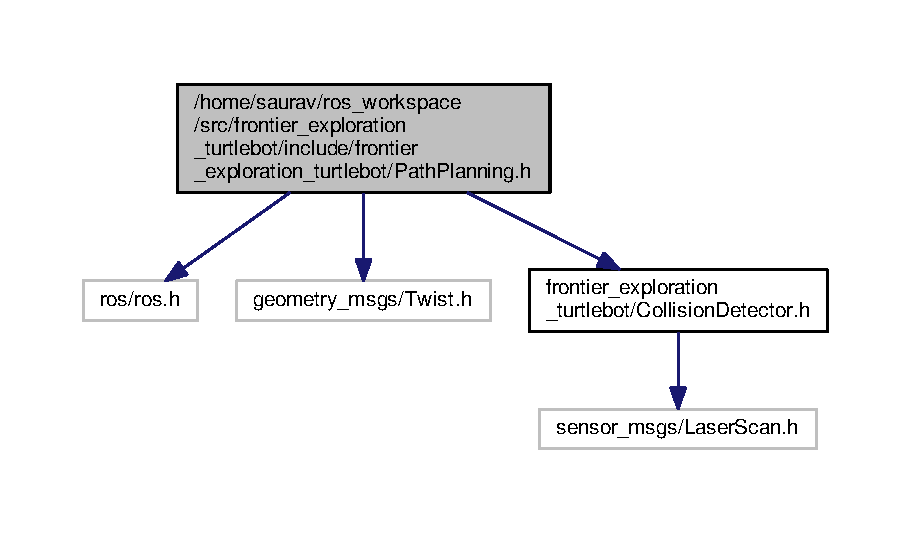
\includegraphics[width=350pt]{PathPlanning_8h__incl}
\end{center}
\end{figure}
This graph shows which files directly or indirectly include this file\+:\nopagebreak
\begin{figure}[H]
\begin{center}
\leavevmode
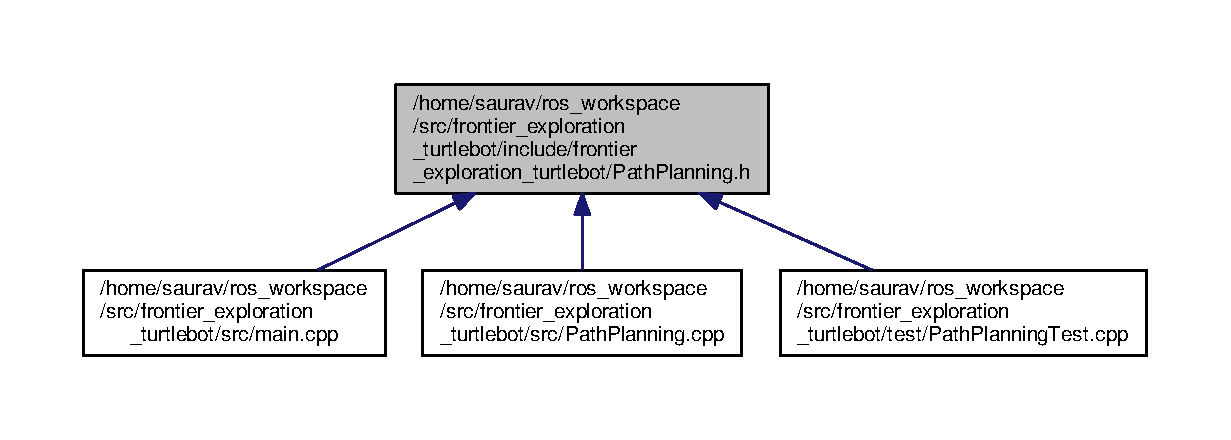
\includegraphics[width=350pt]{PathPlanning_8h__dep__incl}
\end{center}
\end{figure}
\subsection*{Classes}
\begin{DoxyCompactItemize}
\item 
class \hyperlink{classPathPlanning}{Path\+Planning}
\begin{DoxyCompactList}\small\item\em \hyperlink{classPathPlanning}{Path\+Planning} Class class to publish spiral trajectories and linear trajectories and kicks in the colloision avoiding algorithm when required. \end{DoxyCompactList}\end{DoxyCompactItemize}


\subsection{Detailed Description}
\hyperlink{classPathPlanning}{Path\+Planning} class declaration Declares functions to publish spiral trajectories. 

M\+IT License

Copyright (c) 2018 Saimouli Katragadda, Saurav Kumar

Permission is hereby granted, free of charge, to any person obtaining a copy of this software and associated documentation files (the \char`\"{}\+Software\char`\"{}), to deal in the Software without restriction, including without limitation the rights to use, copy, modify, merge, publish, distribute, sublicense, and/or sell copies of the Software, and to permit persons to whom the Software is furnished to do so, subject to the following conditions\+:

The above copyright notice and this permission notice shall be included in all copies or substantial portions of the Software.

T\+HE S\+O\+F\+T\+W\+A\+RE IS P\+R\+O\+V\+I\+D\+ED \char`\"{}\+A\+S I\+S\char`\"{}, W\+I\+T\+H\+O\+UT W\+A\+R\+R\+A\+N\+TY OF A\+NY K\+I\+ND, E\+X\+P\+R\+E\+SS OR I\+M\+P\+L\+I\+ED, I\+N\+C\+L\+U\+D\+I\+NG B\+UT N\+OT L\+I\+M\+I\+T\+ED TO T\+HE W\+A\+R\+R\+A\+N\+T\+I\+ES OF M\+E\+R\+C\+H\+A\+N\+T\+A\+B\+I\+L\+I\+TY, F\+I\+T\+N\+E\+SS F\+OR A P\+A\+R\+T\+I\+C\+U\+L\+AR P\+U\+R\+P\+O\+SE A\+ND N\+O\+N\+I\+N\+F\+R\+I\+N\+G\+E\+M\+E\+NT. IN NO E\+V\+E\+NT S\+H\+A\+LL T\+HE A\+U\+T\+H\+O\+RS OR C\+O\+P\+Y\+R\+I\+G\+HT H\+O\+L\+D\+E\+RS BE L\+I\+A\+B\+LE F\+OR A\+NY C\+L\+A\+IM, D\+A\+M\+A\+G\+ES OR O\+T\+H\+ER L\+I\+A\+B\+I\+L\+I\+TY, W\+H\+E\+T\+H\+ER IN AN A\+C\+T\+I\+ON OF C\+O\+N\+T\+R\+A\+CT, T\+O\+RT OR O\+T\+H\+E\+R\+W\+I\+SE, A\+R\+I\+S\+I\+NG F\+R\+OM, O\+UT OF OR IN C\+O\+N\+N\+E\+C\+T\+I\+ON W\+I\+TH T\+HE S\+O\+F\+T\+W\+A\+RE OR T\+HE U\+SE OR O\+T\+H\+ER D\+E\+A\+L\+I\+N\+GS IN T\+HE S\+O\+F\+T\+W\+A\+RE.

\begin{DoxyAuthor}{Author}
Saimouli Katragadda 

Saurav Kumar 
\end{DoxyAuthor}
\begin{DoxyCopyright}{Copyright}
M\+IT License 
\end{DoxyCopyright}

\hypertarget{CollisionDetector_8cpp}{}\section{/home/saurav/ros\+\_\+workspace/src/frontier\+\_\+exploration\+\_\+turtlebot/src/\+Collision\+Detector.cpp File Reference}
\label{CollisionDetector_8cpp}\index{/home/saurav/ros\+\_\+workspace/src/frontier\+\_\+exploration\+\_\+turtlebot/src/\+Collision\+Detector.\+cpp@{/home/saurav/ros\+\_\+workspace/src/frontier\+\_\+exploration\+\_\+turtlebot/src/\+Collision\+Detector.\+cpp}}


implements the collision\+Detector class methods  


{\ttfamily \#include $<$ros/ros.\+h$>$}\\*
{\ttfamily \#include $<$sensor\+\_\+msgs/\+Laser\+Scan.\+h$>$}\\*
{\ttfamily \#include $<$frontier\+\_\+exploration\+\_\+turtlebot/\+Collision\+Detector.\+h$>$}\\*
{\ttfamily \#include $<$vector$>$}\\*
{\ttfamily \#include $<$algorithm$>$}\\*
Include dependency graph for Collision\+Detector.\+cpp\+:\nopagebreak
\begin{figure}[H]
\begin{center}
\leavevmode
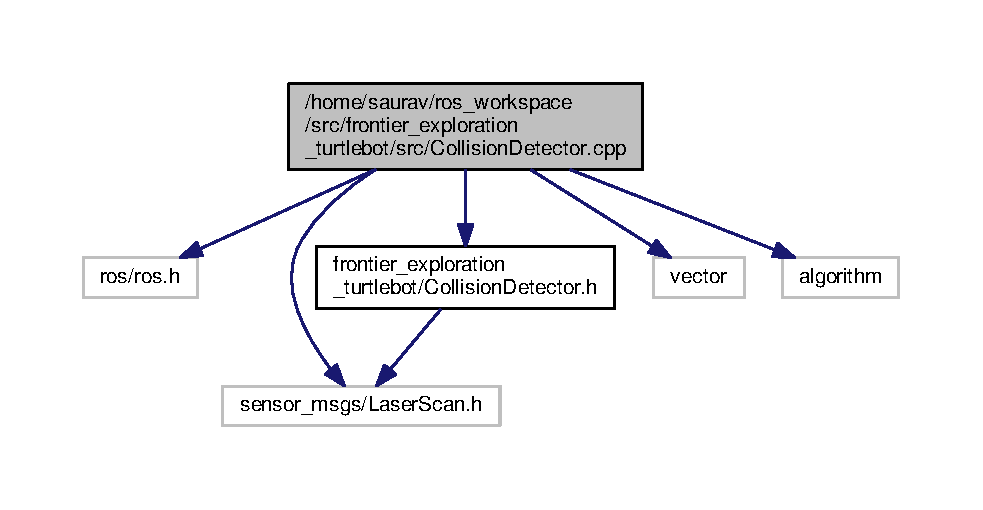
\includegraphics[width=350pt]{CollisionDetector_8cpp__incl}
\end{center}
\end{figure}


\subsection{Detailed Description}
implements the collision\+Detector class methods 

M\+IT License

Copyright (c) 2018 Saimouli Katragadda, Saurav Kumar

Permission is hereby granted, free of charge, to any person obtaining a copy of this software and associated documentation files (the \char`\"{}\+Software\char`\"{}), to deal in the Software without restriction, including without limitation the rights to use, copy, modify, merge, publish, distribute, sublicense, and/or sell copies of the Software, and to permit persons to whom the Software is furnished to do so, subject to the following conditions\+:

The above copyright notice and this permission notice shall be included in all copies or substantial portions of the Software.

T\+HE S\+O\+F\+T\+W\+A\+RE IS P\+R\+O\+V\+I\+D\+ED \char`\"{}\+A\+S I\+S\char`\"{}, W\+I\+T\+H\+O\+UT W\+A\+R\+R\+A\+N\+TY OF A\+NY K\+I\+ND, E\+X\+P\+R\+E\+SS OR I\+M\+P\+L\+I\+ED, I\+N\+C\+L\+U\+D\+I\+NG B\+UT N\+OT L\+I\+M\+I\+T\+ED TO T\+HE W\+A\+R\+R\+A\+N\+T\+I\+ES OF M\+E\+R\+C\+H\+A\+N\+T\+A\+B\+I\+L\+I\+TY, F\+I\+T\+N\+E\+SS F\+OR A P\+A\+R\+T\+I\+C\+U\+L\+AR P\+U\+R\+P\+O\+SE A\+ND N\+O\+N\+I\+N\+F\+R\+I\+N\+G\+E\+M\+E\+NT. IN NO E\+V\+E\+NT S\+H\+A\+LL T\+HE A\+U\+T\+H\+O\+RS OR C\+O\+P\+Y\+R\+I\+G\+HT H\+O\+L\+D\+E\+RS BE L\+I\+A\+B\+LE F\+OR A\+NY C\+L\+A\+IM, D\+A\+M\+A\+G\+ES OR O\+T\+H\+ER L\+I\+A\+B\+I\+L\+I\+TY, W\+H\+E\+T\+H\+ER IN AN A\+C\+T\+I\+ON OF C\+O\+N\+T\+R\+A\+CT, T\+O\+RT OR O\+T\+H\+E\+R\+W\+I\+SE, A\+R\+I\+S\+I\+NG F\+R\+OM, O\+UT OF OR IN C\+O\+N\+N\+E\+C\+T\+I\+ON W\+I\+TH T\+HE S\+O\+F\+T\+W\+A\+RE OR T\+HE U\+SE OR O\+T\+H\+ER D\+E\+A\+L\+I\+N\+GS IN T\+HE S\+O\+F\+T\+W\+A\+RE.

\begin{DoxyAuthor}{Author}
Saimouli Katragadda 

Saurav Kumar 
\end{DoxyAuthor}
\begin{DoxyCopyright}{Copyright}
M\+IT License 
\end{DoxyCopyright}

\hypertarget{src_2main_8cpp}{}\section{/home/saurav/ros\+\_\+workspace/src/frontier\+\_\+exploration\+\_\+turtlebot/src/main.cpp File Reference}
\label{src_2main_8cpp}\index{/home/saurav/ros\+\_\+workspace/src/frontier\+\_\+exploration\+\_\+turtlebot/src/main.\+cpp@{/home/saurav/ros\+\_\+workspace/src/frontier\+\_\+exploration\+\_\+turtlebot/src/main.\+cpp}}
{\ttfamily \#include $<$ros/ros.\+h$>$}\\*
{\ttfamily \#include $<$frontier\+\_\+exploration\+\_\+turtlebot/\+Path\+Planning.\+h$>$}\\*
{\ttfamily \#include $<$frontier\+\_\+exploration\+\_\+turtlebot/\+Collision\+Detector.\+h$>$}\\*
{\ttfamily \#include $<$iostream$>$}\\*
Include dependency graph for main.\+cpp\+:\nopagebreak
\begin{figure}[H]
\begin{center}
\leavevmode
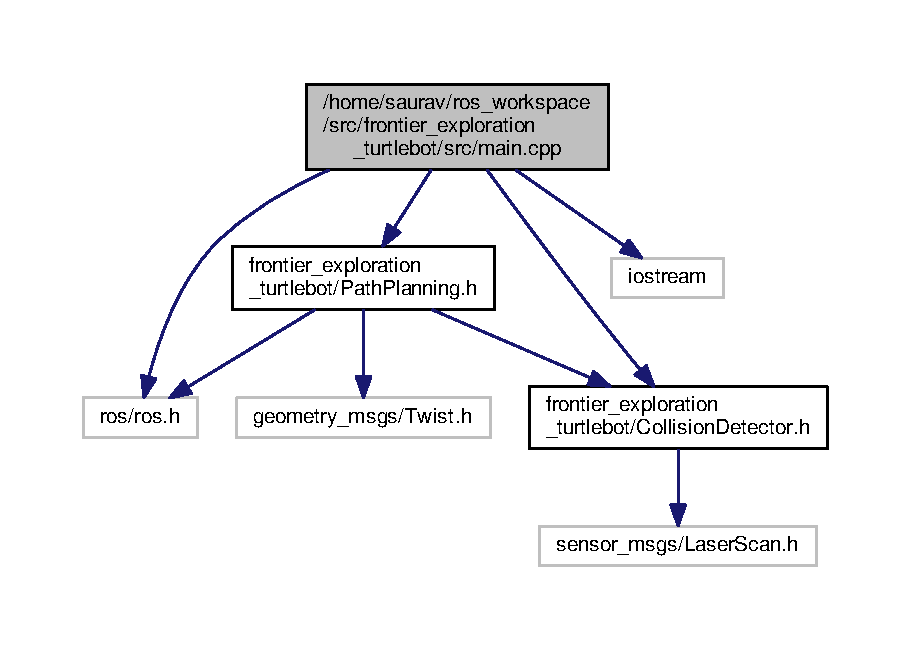
\includegraphics[width=350pt]{src_2main_8cpp__incl}
\end{center}
\end{figure}
\subsection*{Functions}
\begin{DoxyCompactItemize}
\item 
int \hyperlink{src_2main_8cpp_a0ddf1224851353fc92bfbff6f499fa97}{main} (int argc, char $\ast$argv\mbox{[}$\,$\mbox{]})
\begin{DoxyCompactList}\small\item\em main function \end{DoxyCompactList}\end{DoxyCompactItemize}


\subsection{Function Documentation}
\index{src/main.\+cpp@{src/main.\+cpp}!main@{main}}
\index{main@{main}!src/main.\+cpp@{src/main.\+cpp}}
\subsubsection[{\texorpdfstring{main(int argc, char $\ast$argv[])}{main(int argc, char *argv[])}}]{\setlength{\rightskip}{0pt plus 5cm}int main (
\begin{DoxyParamCaption}
\item[{int}]{argc, }
\item[{char $\ast$}]{argv\mbox{[}$\,$\mbox{]}}
\end{DoxyParamCaption}
)}\hypertarget{src_2main_8cpp_a0ddf1224851353fc92bfbff6f499fa97}{}\label{src_2main_8cpp_a0ddf1224851353fc92bfbff6f499fa97}


main function 


\begin{DoxyParams}{Parameters}
{\em argc} & The argc \\
\hline
{\em argv} & The argv \\
\hline
\end{DoxyParams}
\begin{DoxyReturn}{Returns}
int of value zero 
\end{DoxyReturn}


Definition at line 45 of file main.\+cpp.



References Path\+Planning\+::linear\+Path\+Generator(), and Path\+Planning\+::spiral\+Path\+Generator().


\hypertarget{test_2main_8cpp}{}\section{/home/saurav/ros\+\_\+workspace/src/frontier\+\_\+exploration\+\_\+turtlebot/test/main.cpp File Reference}
\label{test_2main_8cpp}\index{/home/saurav/ros\+\_\+workspace/src/frontier\+\_\+exploration\+\_\+turtlebot/test/main.\+cpp@{/home/saurav/ros\+\_\+workspace/src/frontier\+\_\+exploration\+\_\+turtlebot/test/main.\+cpp}}
{\ttfamily \#include $<$ros/ros.\+h$>$}\\*
{\ttfamily \#include $<$gtest/gtest.\+h$>$}\\*
Include dependency graph for main.\+cpp\+:\nopagebreak
\begin{figure}[H]
\begin{center}
\leavevmode
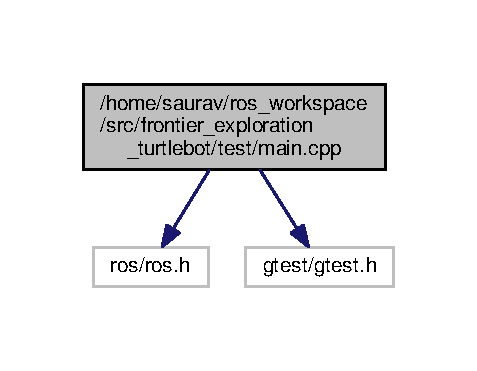
\includegraphics[width=229pt]{test_2main_8cpp__incl}
\end{center}
\end{figure}
\subsection*{Functions}
\begin{DoxyCompactItemize}
\item 
int \hyperlink{test_2main_8cpp_a3c04138a5bfe5d72780bb7e82a18e627}{main} (int argc, char $\ast$$\ast$argv)
\begin{DoxyCompactList}\small\item\em main function for calling tests \end{DoxyCompactList}\end{DoxyCompactItemize}


\subsection{Function Documentation}
\index{test/main.\+cpp@{test/main.\+cpp}!main@{main}}
\index{main@{main}!test/main.\+cpp@{test/main.\+cpp}}
\subsubsection[{\texorpdfstring{main(int argc, char $\ast$$\ast$argv)}{main(int argc, char **argv)}}]{\setlength{\rightskip}{0pt plus 5cm}int main (
\begin{DoxyParamCaption}
\item[{int}]{argc, }
\item[{char $\ast$$\ast$}]{argv}
\end{DoxyParamCaption}
)}\hypertarget{test_2main_8cpp_a3c04138a5bfe5d72780bb7e82a18e627}{}\label{test_2main_8cpp_a3c04138a5bfe5d72780bb7e82a18e627}


main function for calling tests 

M\+IT License

Copyright (c) 2018 Saimouli Katragadda, Saurav Kumar

Permission is hereby granted, free of charge, to any person obtaining a copy of this software and associated documentation files (the \char`\"{}\+Software\char`\"{}), to deal in the Software without restriction, including without limitation the rights to use, copy, modify, merge, publish, distribute, sublicense, and/or sell copies of the Software, and to permit persons to whom the Software is furnished to do so, subject to the following conditions\+:

The above copyright notice and this permission notice shall be included in all copies or substantial portions of the Software.

T\+HE S\+O\+F\+T\+W\+A\+RE IS P\+R\+O\+V\+I\+D\+ED \char`\"{}\+A\+S I\+S\char`\"{}, W\+I\+T\+H\+O\+UT W\+A\+R\+R\+A\+N\+TY OF A\+NY K\+I\+ND, E\+X\+P\+R\+E\+SS OR I\+M\+P\+L\+I\+ED, I\+N\+C\+L\+U\+D\+I\+NG B\+UT N\+OT L\+I\+M\+I\+T\+ED TO T\+HE W\+A\+R\+R\+A\+N\+T\+I\+ES OF M\+E\+R\+C\+H\+A\+N\+T\+A\+B\+I\+L\+I\+TY, F\+I\+T\+N\+E\+SS F\+OR A P\+A\+R\+T\+I\+C\+U\+L\+AR P\+U\+R\+P\+O\+SE A\+ND N\+O\+N\+I\+N\+F\+R\+I\+N\+G\+E\+M\+E\+NT. IN NO E\+V\+E\+NT S\+H\+A\+LL T\+HE A\+U\+T\+H\+O\+RS OR C\+O\+P\+Y\+R\+I\+G\+HT H\+O\+L\+D\+E\+RS BE L\+I\+A\+B\+LE F\+OR A\+NY C\+L\+A\+IM, D\+A\+M\+A\+G\+ES OR O\+T\+H\+ER L\+I\+A\+B\+I\+L\+I\+TY, W\+H\+E\+T\+H\+ER IN AN A\+C\+T\+I\+ON OF C\+O\+N\+T\+R\+A\+CT, T\+O\+RT OR O\+T\+H\+E\+R\+W\+I\+SE, A\+R\+I\+S\+I\+NG F\+R\+OM, O\+UT OF OR IN C\+O\+N\+N\+E\+C\+T\+I\+ON W\+I\+TH T\+HE S\+O\+F\+T\+W\+A\+RE OR T\+HE U\+SE OR O\+T\+H\+ER D\+E\+A\+L\+I\+N\+GS IN T\+HE S\+O\+F\+T\+W\+A\+RE. 
\begin{DoxyParams}{Parameters}
{\em argc} & int \\
\hline
{\em argv} & character array \\
\hline
\end{DoxyParams}
\begin{DoxyReturn}{Returns}
0 on successful exit 
\end{DoxyReturn}


Definition at line 35 of file main.\+cpp.


\hypertarget{PathPlanning_8cpp}{}\section{/home/saurav/ros\+\_\+workspace/src/frontier\+\_\+exploration\+\_\+turtlebot/src/\+Path\+Planning.cpp File Reference}
\label{PathPlanning_8cpp}\index{/home/saurav/ros\+\_\+workspace/src/frontier\+\_\+exploration\+\_\+turtlebot/src/\+Path\+Planning.\+cpp@{/home/saurav/ros\+\_\+workspace/src/frontier\+\_\+exploration\+\_\+turtlebot/src/\+Path\+Planning.\+cpp}}


implements the \hyperlink{classPathPlanning}{Path\+Planning} class methods  


{\ttfamily \#include $<$ros/ros.\+h$>$}\\*
{\ttfamily \#include $<$sensor\+\_\+msgs/\+Laser\+Scan.\+h$>$}\\*
{\ttfamily \#include $<$geometry\+\_\+msgs/\+Twist.\+h$>$}\\*
{\ttfamily \#include $<$frontier\+\_\+exploration\+\_\+turtlebot/\+Collision\+Detector.\+h$>$}\\*
{\ttfamily \#include $<$frontier\+\_\+exploration\+\_\+turtlebot/\+Path\+Planning.\+h$>$}\\*
Include dependency graph for Path\+Planning.\+cpp\+:\nopagebreak
\begin{figure}[H]
\begin{center}
\leavevmode
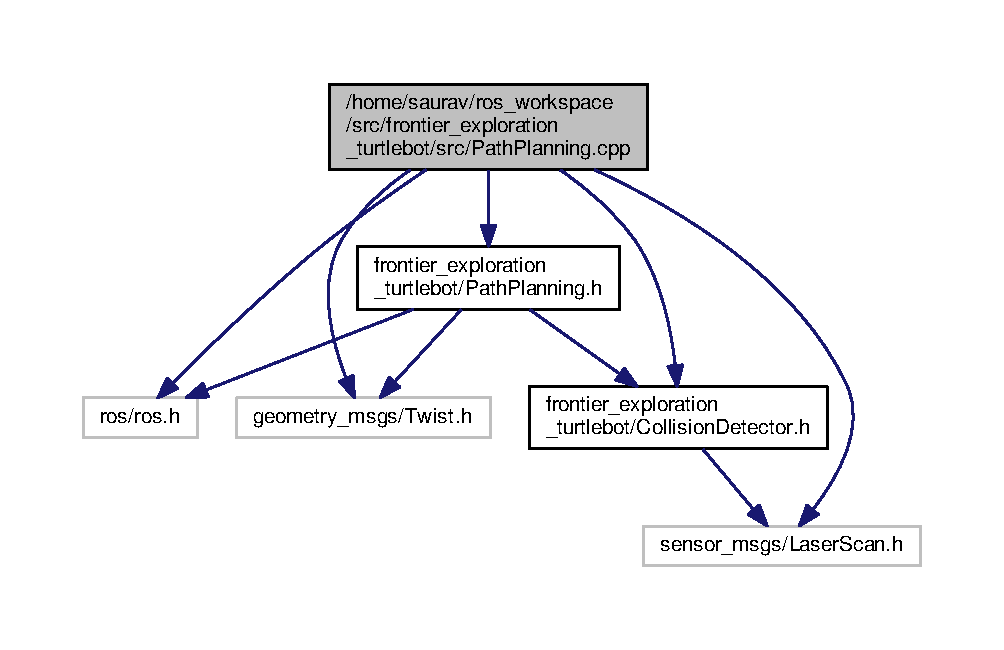
\includegraphics[width=350pt]{PathPlanning_8cpp__incl}
\end{center}
\end{figure}


\subsection{Detailed Description}
implements the \hyperlink{classPathPlanning}{Path\+Planning} class methods 

M\+IT License

Copyright (c) 2018 Saimouli Katragadda, Saurav Kumar

Permission is hereby granted, free of charge, to any person obtaining a copy of this software and associated documentation files (the \char`\"{}\+Software\char`\"{}), to deal in the Software without restriction, including without limitation the rights to use, copy, modify, merge, publish, distribute, sublicense, and/or sell copies of the Software, and to permit persons to whom the Software is furnished to do so, subject to the following conditions\+:

The above copyright notice and this permission notice shall be included in all copies or substantial portions of the Software.

T\+HE S\+O\+F\+T\+W\+A\+RE IS P\+R\+O\+V\+I\+D\+ED \char`\"{}\+A\+S I\+S\char`\"{}, W\+I\+T\+H\+O\+UT W\+A\+R\+R\+A\+N\+TY OF A\+NY K\+I\+ND, E\+X\+P\+R\+E\+SS OR I\+M\+P\+L\+I\+ED, I\+N\+C\+L\+U\+D\+I\+NG B\+UT N\+OT L\+I\+M\+I\+T\+ED TO T\+HE W\+A\+R\+R\+A\+N\+T\+I\+ES OF M\+E\+R\+C\+H\+A\+N\+T\+A\+B\+I\+L\+I\+TY, F\+I\+T\+N\+E\+SS F\+OR A P\+A\+R\+T\+I\+C\+U\+L\+AR P\+U\+R\+P\+O\+SE A\+ND N\+O\+N\+I\+N\+F\+R\+I\+N\+G\+E\+M\+E\+NT. IN NO E\+V\+E\+NT S\+H\+A\+LL T\+HE A\+U\+T\+H\+O\+RS OR C\+O\+P\+Y\+R\+I\+G\+HT H\+O\+L\+D\+E\+RS BE L\+I\+A\+B\+LE F\+OR A\+NY C\+L\+A\+IM, D\+A\+M\+A\+G\+ES OR O\+T\+H\+ER L\+I\+A\+B\+I\+L\+I\+TY, W\+H\+E\+T\+H\+ER IN AN A\+C\+T\+I\+ON OF C\+O\+N\+T\+R\+A\+CT, T\+O\+RT OR O\+T\+H\+E\+R\+W\+I\+SE, A\+R\+I\+S\+I\+NG F\+R\+OM, O\+UT OF OR IN C\+O\+N\+N\+E\+C\+T\+I\+ON W\+I\+TH T\+HE S\+O\+F\+T\+W\+A\+RE OR T\+HE U\+SE OR O\+T\+H\+ER D\+E\+A\+L\+I\+N\+GS IN T\+HE S\+O\+F\+T\+W\+A\+RE.

\begin{DoxyAuthor}{Author}
Saimouli Katragadda 

Saurav Kumar 
\end{DoxyAuthor}
\begin{DoxyCopyright}{Copyright}
M\+IT License 
\end{DoxyCopyright}

\hypertarget{CollisionDetectorTest_8cpp}{}\section{/home/saurav/ros\+\_\+workspace/src/frontier\+\_\+exploration\+\_\+turtlebot/test/\+Collision\+Detector\+Test.cpp File Reference}
\label{CollisionDetectorTest_8cpp}\index{/home/saurav/ros\+\_\+workspace/src/frontier\+\_\+exploration\+\_\+turtlebot/test/\+Collision\+Detector\+Test.\+cpp@{/home/saurav/ros\+\_\+workspace/src/frontier\+\_\+exploration\+\_\+turtlebot/test/\+Collision\+Detector\+Test.\+cpp}}


Tests the collision\+Detector class methods.  


{\ttfamily \#include $<$ros/ros.\+h$>$}\\*
{\ttfamily \#include $<$sensor\+\_\+msgs/\+Laser\+Scan.\+h$>$}\\*
{\ttfamily \#include $<$frontier\+\_\+exploration\+\_\+turtlebot/\+Collision\+Detector.\+h$>$}\\*
{\ttfamily \#include $<$gtest/gtest.\+h$>$}\\*
{\ttfamily \#include $<$iostream$>$}\\*
Include dependency graph for Collision\+Detector\+Test.\+cpp\+:\nopagebreak
\begin{figure}[H]
\begin{center}
\leavevmode
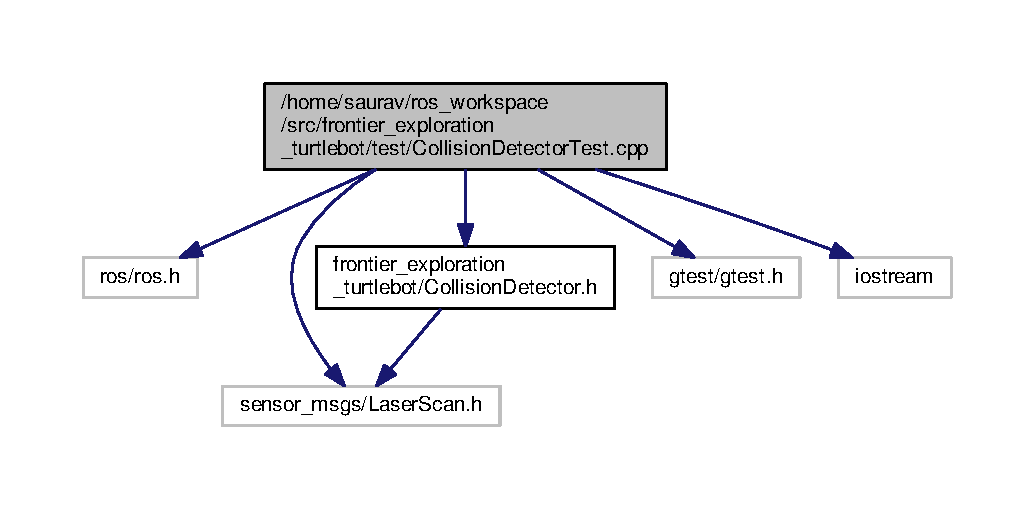
\includegraphics[width=350pt]{CollisionDetectorTest_8cpp__incl}
\end{center}
\end{figure}
\subsection*{Functions}
\begin{DoxyCompactItemize}
\item 
\hyperlink{CollisionDetectorTest_8cpp_a29866386b12e9d650cd4236387bb880b}{T\+E\+ST} (Collision\+Detector\+Test, Collision\+Detector\+Test)
\begin{DoxyCompactList}\small\item\em Tests constructor of the class \hyperlink{classCollisionDetector}{Collision\+Detector}. \end{DoxyCompactList}\item 
\hyperlink{CollisionDetectorTest_8cpp_ad5710e780c93d298f920f44517e7ba38}{T\+E\+ST} (Collision\+Detector\+Test, laser\+Callback\+Test)
\begin{DoxyCompactList}\small\item\em Tests laser\+Callback method of the class \hyperlink{classCollisionDetector}{Collision\+Detector}. \end{DoxyCompactList}\end{DoxyCompactItemize}


\subsection{Detailed Description}
Tests the collision\+Detector class methods. 

M\+IT License

Copyright (c) 2018 Saimouli Katragadda, Saurav Kumar

Permission is hereby granted, free of charge, to any person obtaining a copy of this software and associated documentation files (the \char`\"{}\+Software\char`\"{}), to deal in the Software without restriction, including without limitation the rights to use, copy, modify, merge, publish, distribute, sublicense, and/or sell copies of the Software, and to permit persons to whom the Software is furnished to do so, subject to the following conditions\+:

The above copyright notice and this permission notice shall be included in all copies or substantial portions of the Software.

T\+HE S\+O\+F\+T\+W\+A\+RE IS P\+R\+O\+V\+I\+D\+ED \char`\"{}\+A\+S I\+S\char`\"{}, W\+I\+T\+H\+O\+UT W\+A\+R\+R\+A\+N\+TY OF A\+NY K\+I\+ND, E\+X\+P\+R\+E\+SS OR I\+M\+P\+L\+I\+ED, I\+N\+C\+L\+U\+D\+I\+NG B\+UT N\+OT L\+I\+M\+I\+T\+ED TO T\+HE W\+A\+R\+R\+A\+N\+T\+I\+ES OF M\+E\+R\+C\+H\+A\+N\+T\+A\+B\+I\+L\+I\+TY, F\+I\+T\+N\+E\+SS F\+OR A P\+A\+R\+T\+I\+C\+U\+L\+AR P\+U\+R\+P\+O\+SE A\+ND N\+O\+N\+I\+N\+F\+R\+I\+N\+G\+E\+M\+E\+NT. IN NO E\+V\+E\+NT S\+H\+A\+LL T\+HE A\+U\+T\+H\+O\+RS OR C\+O\+P\+Y\+R\+I\+G\+HT H\+O\+L\+D\+E\+RS BE L\+I\+A\+B\+LE F\+OR A\+NY C\+L\+A\+IM, D\+A\+M\+A\+G\+ES OR O\+T\+H\+ER L\+I\+A\+B\+I\+L\+I\+TY, W\+H\+E\+T\+H\+ER IN AN A\+C\+T\+I\+ON OF C\+O\+N\+T\+R\+A\+CT, T\+O\+RT OR O\+T\+H\+E\+R\+W\+I\+SE, A\+R\+I\+S\+I\+NG F\+R\+OM, O\+UT OF OR IN C\+O\+N\+N\+E\+C\+T\+I\+ON W\+I\+TH T\+HE S\+O\+F\+T\+W\+A\+RE OR T\+HE U\+SE OR O\+T\+H\+ER D\+E\+A\+L\+I\+N\+GS IN T\+HE S\+O\+F\+T\+W\+A\+RE.

\begin{DoxyAuthor}{Author}
Saimouli Katragadda 

Saurav Kumar 
\end{DoxyAuthor}
\begin{DoxyCopyright}{Copyright}
M\+IT License 
\end{DoxyCopyright}


\subsection{Function Documentation}
\index{Collision\+Detector\+Test.\+cpp@{Collision\+Detector\+Test.\+cpp}!T\+E\+ST@{T\+E\+ST}}
\index{T\+E\+ST@{T\+E\+ST}!Collision\+Detector\+Test.\+cpp@{Collision\+Detector\+Test.\+cpp}}
\subsubsection[{\texorpdfstring{T\+E\+S\+T(\+Collision\+Detector\+Test, Collision\+Detector\+Test)}{TEST(CollisionDetectorTest, CollisionDetectorTest)}}]{\setlength{\rightskip}{0pt plus 5cm}T\+E\+ST (
\begin{DoxyParamCaption}
\item[{Collision\+Detector\+Test}]{, }
\item[{Collision\+Detector\+Test}]{}
\end{DoxyParamCaption}
)}\hypertarget{CollisionDetectorTest_8cpp_a29866386b12e9d650cd4236387bb880b}{}\label{CollisionDetectorTest_8cpp_a29866386b12e9d650cd4236387bb880b}


Tests constructor of the class \hyperlink{classCollisionDetector}{Collision\+Detector}. 


\begin{DoxyParams}{Parameters}
{\em Collision\+Detector\+Test} & gtest framework \\
\hline
{\em Collision\+Detector\+Test} & Name of the test \\
\hline
\end{DoxyParams}
\begin{DoxyReturn}{Returns}
none 
\end{DoxyReturn}


Definition at line 46 of file Collision\+Detector\+Test.\+cpp.



References Collision\+Detector\+::check\+Obstacles().

\index{Collision\+Detector\+Test.\+cpp@{Collision\+Detector\+Test.\+cpp}!T\+E\+ST@{T\+E\+ST}}
\index{T\+E\+ST@{T\+E\+ST}!Collision\+Detector\+Test.\+cpp@{Collision\+Detector\+Test.\+cpp}}
\subsubsection[{\texorpdfstring{T\+E\+S\+T(\+Collision\+Detector\+Test, laser\+Callback\+Test)}{TEST(CollisionDetectorTest, laserCallbackTest)}}]{\setlength{\rightskip}{0pt plus 5cm}T\+E\+ST (
\begin{DoxyParamCaption}
\item[{Collision\+Detector\+Test}]{, }
\item[{laser\+Callback\+Test}]{}
\end{DoxyParamCaption}
)}\hypertarget{CollisionDetectorTest_8cpp_ad5710e780c93d298f920f44517e7ba38}{}\label{CollisionDetectorTest_8cpp_ad5710e780c93d298f920f44517e7ba38}


Tests laser\+Callback method of the class \hyperlink{classCollisionDetector}{Collision\+Detector}. 


\begin{DoxyParams}{Parameters}
{\em Collision\+Detector\+Test} & gtest framework \\
\hline
{\em distance\+Callback\+Test} & Name of the test \\
\hline
\end{DoxyParams}
\begin{DoxyReturn}{Returns}
none 
\end{DoxyReturn}


Definition at line 58 of file Collision\+Detector\+Test.\+cpp.



References Collision\+Detector\+::check\+Obstacles(), and Collision\+Detector\+::laser\+Callback().


\hypertarget{PathPlanningTest_8cpp}{}\section{/home/saurav/ros\+\_\+workspace/src/frontier\+\_\+exploration\+\_\+turtlebot/test/\+Path\+Planning\+Test.cpp File Reference}
\label{PathPlanningTest_8cpp}\index{/home/saurav/ros\+\_\+workspace/src/frontier\+\_\+exploration\+\_\+turtlebot/test/\+Path\+Planning\+Test.\+cpp@{/home/saurav/ros\+\_\+workspace/src/frontier\+\_\+exploration\+\_\+turtlebot/test/\+Path\+Planning\+Test.\+cpp}}


Tests the \hyperlink{classPathPlanning}{Path\+Planning} class methods.  


{\ttfamily \#include $<$ros/ros.\+h$>$}\\*
{\ttfamily \#include $<$sensor\+\_\+msgs/\+Laser\+Scan.\+h$>$}\\*
{\ttfamily \#include $<$geometry\+\_\+msgs/\+Twist.\+h$>$}\\*
{\ttfamily \#include $<$gtest/gtest.\+h$>$}\\*
{\ttfamily \#include $<$frontier\+\_\+exploration\+\_\+turtlebot/\+Collision\+Detector.\+h$>$}\\*
{\ttfamily \#include $<$frontier\+\_\+exploration\+\_\+turtlebot/\+Path\+Planning.\+h$>$}\\*
Include dependency graph for Path\+Planning\+Test.\+cpp\+:\nopagebreak
\begin{figure}[H]
\begin{center}
\leavevmode
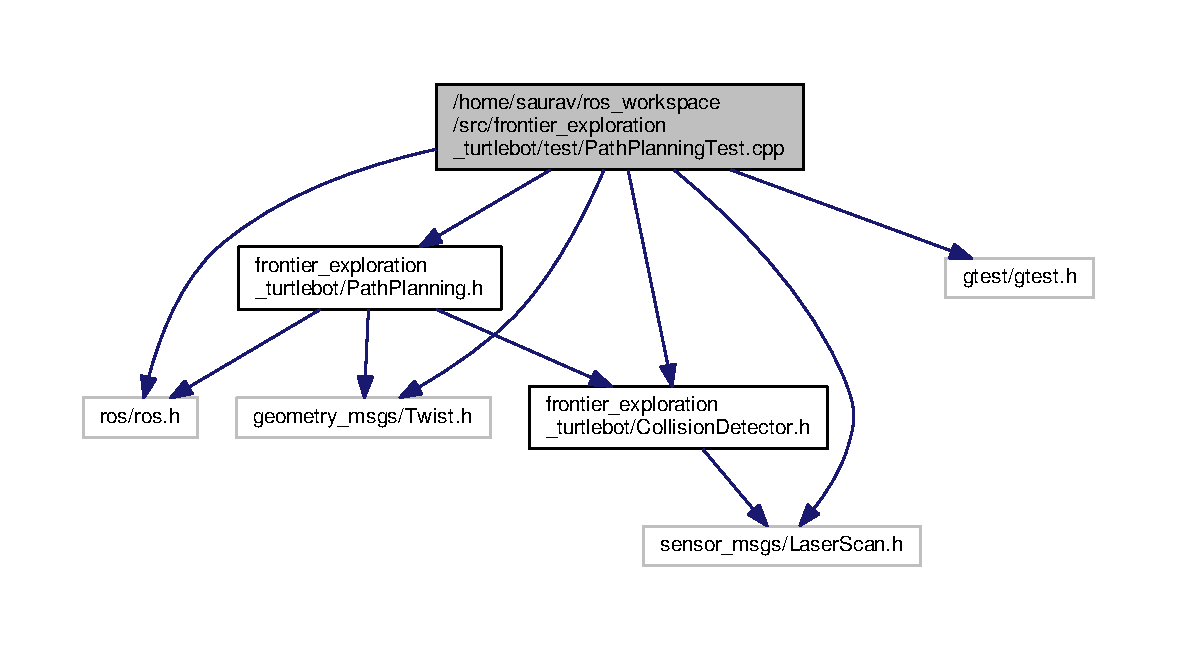
\includegraphics[width=350pt]{PathPlanningTest_8cpp__incl}
\end{center}
\end{figure}
\subsection*{Functions}
\begin{DoxyCompactItemize}
\item 
void \hyperlink{PathPlanningTest_8cpp_ac668b514bd2d48d7e71fc2be8088acc9}{test\+Callback} (const geometry\+\_\+msgs\+::\+Twist msg)
\begin{DoxyCompactList}\small\item\em global function to store the twist msg value to global float variabls \end{DoxyCompactList}\item 
\hyperlink{PathPlanningTest_8cpp_a6dfa97f8e1249613431b507db7114cee}{T\+E\+ST} (Path\+Planning\+Test, Initialization\+Error\+Test)
\begin{DoxyCompactList}\small\item\em Tests for initialization. \end{DoxyCompactList}\item 
\hyperlink{PathPlanningTest_8cpp_ab270fed7f2dc84e46052f9f05c717312}{T\+E\+ST} (Path\+Planning\+Test, spiral\+Path\+Generator\+Test)
\begin{DoxyCompactList}\small\item\em Tests spiral\+Path\+Generator method of the class \hyperlink{classPathPlanning}{Path\+Planning}. \end{DoxyCompactList}\item 
\hyperlink{PathPlanningTest_8cpp_a58aa1b64ae54ee0d74f86df79630be25}{T\+E\+ST} (Path\+Planning\+Test, linear\+Path\+Generator\+Test)
\begin{DoxyCompactList}\small\item\em Tests linear\+Path\+Generator method of the class \hyperlink{classPathPlanning}{Path\+Planning}. \end{DoxyCompactList}\end{DoxyCompactItemize}
\subsection*{Variables}
\begin{DoxyCompactItemize}
\item 
float \hyperlink{PathPlanningTest_8cpp_a51b71b417294ba319a3c8fa6dd5782a8}{linX} = 0.\+0
\item 
float \hyperlink{PathPlanningTest_8cpp_a2c4fd2faa661a6f48012086f35c6015c}{angZ}
\end{DoxyCompactItemize}


\subsection{Detailed Description}
Tests the \hyperlink{classPathPlanning}{Path\+Planning} class methods. 

M\+IT License

Copyright (c) 2018 Saimouli Katragadda, Saurav Kumar

Permission is hereby granted, free of charge, to any person obtaining a copy of this software and associated documentation files (the \char`\"{}\+Software\char`\"{}), to deal in the Software without restriction, including without limitation the rights to use, copy, modify, merge, publish, distribute, sublicense, and/or sell copies of the Software, and to permit persons to whom the Software is furnished to do so, subject to the following conditions\+:

The above copyright notice and this permission notice shall be included in all copies or substantial portions of the Software.

T\+HE S\+O\+F\+T\+W\+A\+RE IS P\+R\+O\+V\+I\+D\+ED \char`\"{}\+A\+S I\+S\char`\"{}, W\+I\+T\+H\+O\+UT W\+A\+R\+R\+A\+N\+TY OF A\+NY K\+I\+ND, E\+X\+P\+R\+E\+SS OR I\+M\+P\+L\+I\+ED, I\+N\+C\+L\+U\+D\+I\+NG B\+UT N\+OT L\+I\+M\+I\+T\+ED TO T\+HE W\+A\+R\+R\+A\+N\+T\+I\+ES OF M\+E\+R\+C\+H\+A\+N\+T\+A\+B\+I\+L\+I\+TY, F\+I\+T\+N\+E\+SS F\+OR A P\+A\+R\+T\+I\+C\+U\+L\+AR P\+U\+R\+P\+O\+SE A\+ND N\+O\+N\+I\+N\+F\+R\+I\+N\+G\+E\+M\+E\+NT. IN NO E\+V\+E\+NT S\+H\+A\+LL T\+HE A\+U\+T\+H\+O\+RS OR C\+O\+P\+Y\+R\+I\+G\+HT H\+O\+L\+D\+E\+RS BE L\+I\+A\+B\+LE F\+OR A\+NY C\+L\+A\+IM, D\+A\+M\+A\+G\+ES OR O\+T\+H\+ER L\+I\+A\+B\+I\+L\+I\+TY, W\+H\+E\+T\+H\+ER IN AN A\+C\+T\+I\+ON OF C\+O\+N\+T\+R\+A\+CT, T\+O\+RT OR O\+T\+H\+E\+R\+W\+I\+SE, A\+R\+I\+S\+I\+NG F\+R\+OM, O\+UT OF OR IN C\+O\+N\+N\+E\+C\+T\+I\+ON W\+I\+TH T\+HE S\+O\+F\+T\+W\+A\+RE OR T\+HE U\+SE OR O\+T\+H\+ER D\+E\+A\+L\+I\+N\+GS IN T\+HE S\+O\+F\+T\+W\+A\+RE.

\begin{DoxyAuthor}{Author}
Saimouli Katragadda 

Saurav Kumar 
\end{DoxyAuthor}
\begin{DoxyCopyright}{Copyright}
M\+IT License 
\end{DoxyCopyright}


\subsection{Function Documentation}
\index{Path\+Planning\+Test.\+cpp@{Path\+Planning\+Test.\+cpp}!T\+E\+ST@{T\+E\+ST}}
\index{T\+E\+ST@{T\+E\+ST}!Path\+Planning\+Test.\+cpp@{Path\+Planning\+Test.\+cpp}}
\subsubsection[{\texorpdfstring{T\+E\+S\+T(\+Path\+Planning\+Test, Initialization\+Error\+Test)}{TEST(PathPlanningTest, InitializationErrorTest)}}]{\setlength{\rightskip}{0pt plus 5cm}T\+E\+ST (
\begin{DoxyParamCaption}
\item[{Path\+Planning\+Test}]{, }
\item[{Initialization\+Error\+Test}]{}
\end{DoxyParamCaption}
)}\hypertarget{PathPlanningTest_8cpp_a6dfa97f8e1249613431b507db7114cee}{}\label{PathPlanningTest_8cpp_a6dfa97f8e1249613431b507db7114cee}


Tests for initialization. 


\begin{DoxyParams}{Parameters}
{\em Path\+Planning\+Test} & gtest framework \\
\hline
{\em Initialization\+Error\+Test} & Name of the test \\
\hline
\end{DoxyParams}


Definition at line 59 of file Path\+Planning\+Test.\+cpp.

\index{Path\+Planning\+Test.\+cpp@{Path\+Planning\+Test.\+cpp}!T\+E\+ST@{T\+E\+ST}}
\index{T\+E\+ST@{T\+E\+ST}!Path\+Planning\+Test.\+cpp@{Path\+Planning\+Test.\+cpp}}
\subsubsection[{\texorpdfstring{T\+E\+S\+T(\+Path\+Planning\+Test, spiral\+Path\+Generator\+Test)}{TEST(PathPlanningTest, spiralPathGeneratorTest)}}]{\setlength{\rightskip}{0pt plus 5cm}T\+E\+ST (
\begin{DoxyParamCaption}
\item[{Path\+Planning\+Test}]{, }
\item[{spiral\+Path\+Generator\+Test}]{}
\end{DoxyParamCaption}
)}\hypertarget{PathPlanningTest_8cpp_ab270fed7f2dc84e46052f9f05c717312}{}\label{PathPlanningTest_8cpp_ab270fed7f2dc84e46052f9f05c717312}


Tests spiral\+Path\+Generator method of the class \hyperlink{classPathPlanning}{Path\+Planning}. 


\begin{DoxyParams}{Parameters}
{\em Path\+Planning\+Test} & gtest framework \\
\hline
{\em spiral\+Path\+Generator\+Test} & Name of the test \\
\hline
\end{DoxyParams}
\begin{DoxyReturn}{Returns}
none 
\end{DoxyReturn}


Definition at line 70 of file Path\+Planning\+Test.\+cpp.



References angZ, linX, Path\+Planning\+::spiral\+Path\+Generator(), and test\+Callback().

\index{Path\+Planning\+Test.\+cpp@{Path\+Planning\+Test.\+cpp}!T\+E\+ST@{T\+E\+ST}}
\index{T\+E\+ST@{T\+E\+ST}!Path\+Planning\+Test.\+cpp@{Path\+Planning\+Test.\+cpp}}
\subsubsection[{\texorpdfstring{T\+E\+S\+T(\+Path\+Planning\+Test, linear\+Path\+Generator\+Test)}{TEST(PathPlanningTest, linearPathGeneratorTest)}}]{\setlength{\rightskip}{0pt plus 5cm}T\+E\+ST (
\begin{DoxyParamCaption}
\item[{Path\+Planning\+Test}]{, }
\item[{linear\+Path\+Generator\+Test}]{}
\end{DoxyParamCaption}
)}\hypertarget{PathPlanningTest_8cpp_a58aa1b64ae54ee0d74f86df79630be25}{}\label{PathPlanningTest_8cpp_a58aa1b64ae54ee0d74f86df79630be25}


Tests linear\+Path\+Generator method of the class \hyperlink{classPathPlanning}{Path\+Planning}. 


\begin{DoxyParams}{Parameters}
{\em Path\+Planning\+Test} & gtest framework \\
\hline
{\em linear\+Path\+Generator\+Test} & Name of the test \\
\hline
\end{DoxyParams}
\begin{DoxyReturn}{Returns}
none 
\end{DoxyReturn}


Definition at line 116 of file Path\+Planning\+Test.\+cpp.



References angZ, Path\+Planning\+::linear\+Path\+Generator(), linX, and test\+Callback().

\index{Path\+Planning\+Test.\+cpp@{Path\+Planning\+Test.\+cpp}!test\+Callback@{test\+Callback}}
\index{test\+Callback@{test\+Callback}!Path\+Planning\+Test.\+cpp@{Path\+Planning\+Test.\+cpp}}
\subsubsection[{\texorpdfstring{test\+Callback(const geometry\+\_\+msgs\+::\+Twist msg)}{testCallback(const geometry_msgs::Twist msg)}}]{\setlength{\rightskip}{0pt plus 5cm}void test\+Callback (
\begin{DoxyParamCaption}
\item[{const geometry\+\_\+msgs\+::\+Twist}]{msg}
\end{DoxyParamCaption}
)}\hypertarget{PathPlanningTest_8cpp_ac668b514bd2d48d7e71fc2be8088acc9}{}\label{PathPlanningTest_8cpp_ac668b514bd2d48d7e71fc2be8088acc9}


global function to store the twist msg value to global float variabls 


\begin{DoxyParams}{Parameters}
{\em const} & geometry\+\_\+msgs\+::\+Twist msg \\
\hline
\end{DoxyParams}
\begin{DoxyReturn}{Returns}
void 
\end{DoxyReturn}


Definition at line 49 of file Path\+Planning\+Test.\+cpp.



References angZ, and linX.



Referenced by T\+E\+S\+T().



\subsection{Variable Documentation}
\index{Path\+Planning\+Test.\+cpp@{Path\+Planning\+Test.\+cpp}!angZ@{angZ}}
\index{angZ@{angZ}!Path\+Planning\+Test.\+cpp@{Path\+Planning\+Test.\+cpp}}
\subsubsection[{\texorpdfstring{angZ}{angZ}}]{\setlength{\rightskip}{0pt plus 5cm}float angZ}\hypertarget{PathPlanningTest_8cpp_a2c4fd2faa661a6f48012086f35c6015c}{}\label{PathPlanningTest_8cpp_a2c4fd2faa661a6f48012086f35c6015c}


Definition at line 42 of file Path\+Planning\+Test.\+cpp.



Referenced by T\+E\+S\+T(), and test\+Callback().

\index{Path\+Planning\+Test.\+cpp@{Path\+Planning\+Test.\+cpp}!linX@{linX}}
\index{linX@{linX}!Path\+Planning\+Test.\+cpp@{Path\+Planning\+Test.\+cpp}}
\subsubsection[{\texorpdfstring{linX}{linX}}]{\setlength{\rightskip}{0pt plus 5cm}float linX = 0.\+0}\hypertarget{PathPlanningTest_8cpp_a51b71b417294ba319a3c8fa6dd5782a8}{}\label{PathPlanningTest_8cpp_a51b71b417294ba319a3c8fa6dd5782a8}


Definition at line 42 of file Path\+Planning\+Test.\+cpp.



Referenced by T\+E\+S\+T(), and test\+Callback().


%--- End generated contents ---

% Index
\backmatter
\newpage
\phantomsection
\clearemptydoublepage
\addcontentsline{toc}{chapter}{Index}
\printindex

\end{document}
